\documentclass[12pt, letterpaper, twoside]{article}
\usepackage{nopageno,epsfig, amsmath, amssymb}
\usepackage{physics}
\usepackage{mathtools}
\usepackage{hyperref}
\usepackage{xcolor}
\hypersetup{
    colorlinks,
    linkcolor={blue},
    citecolor={blue},
    urlcolor={blue}
}
\usepackage{empheq}
\usepackage{wrapfig}

\usepackage[letterpaper,
            margin=0.8in]{geometry}

\newcommand{\psetnum}{1}
\newcommand{\class}{ASTR 558 - Exoplanets}

\newcommand{\tomtitle}{
    \noindent {\LARGE \fontfamily{cmr}\selectfont \textbf{\class}} \hfill \\[1\baselineskip]
    \noindent {\large \fontfamily{cmr}\selectfont Problem Set \psetnum \hfill \textsc{Tom Wagg}}\\[0.5\baselineskip]
    {\fontfamily{cmr}\selectfont \textit{\today}}\\[2\baselineskip]
}

\title{\class : Problem Set \psetnum}
\author{\textbf{Tom Wagg}}

\newcommand{\question}[1]{{\noindent \it #1}}
\newcommand{\answer}[1]{
    \par\noindent\rule{\textwidth}{0.4pt}#1\vspace{0.5cm}
}
\newcommand{\todo}[1]{{\color{red}\begin{center}TODO: #1\end{center}}}

% custom function for adding units
\makeatletter
\newcommand{\unit}[1]{%
    \,\mathrm{#1}\checknextarg}
\newcommand{\checknextarg}{\@ifnextchar\bgroup{\gobblenextarg}{}}
\newcommand{\gobblenextarg}[1]{\,\mathrm{#1}\@ifnextchar\bgroup{\gobblenextarg}{}}
\makeatother

\newcommand{\avg}[1]{\left\langle #1 \right\rangle}
\newcommand{\angstrom}{\mbox{\normalfont\AA}}
\allowdisplaybreaks

\begin{document}

\tomtitle

\noindent All code that I used for this homework can be found in \href{https://www.github.com/TomWagg/uw-grad-classes/blob/main/558_exoplanets/pset1/planet_finder.py}{\texttt{planet\_finder.py}}. The various functions handle the different questions and if you want to re-run it then you can just run \texttt{python planet\_finder.py} and it'll take about 10 minutes.\\

\question{\textbf{Q1. Kepler Solver}}
\answer{
    I wrote a solver for Kepler's equation in the function \texttt{solve\_kepler\_equation()} and validated it by running 10,000 checks by putting the resulting eccentric anomaly back into the Kepler equation (this is done in \texttt{test\_kepler\_solver()}).
}

\question{\textbf{Q2. Radial Velocity Equation}}
\answer{
    This is implemented in \texttt{radial\_velocity()}. It is formulated slightly different from class because I figured I could simplify some of the trig by turning
    \begin{equation}
        v_{rv} = k_* \qty[ \cos f(t) \cos \omega - \sin f(t) \sin \omega + e \cos \omega ] + \gamma
    \end{equation}
    into the following by using the addition identities.
    \begin{equation}
        v_{rv} = k_* \qty[ \cos (f(t) + \omega) + e \cos \omega ] + \gamma
    \end{equation}
}

\question{\textbf{Q3. Find planet period}}
\answer{
    I followed the method that Eric demonstrated in class in order to find the period. I chose a grid of periods over which to search and, for each of them, folded the data based on this period, sorted it by phase and then calculate the sum of the square of the difference between adjacent points. I plot this in a periodogram in Figure 1.
    \begin{figure}
        \centering
        % \includegraphics[width=\textwidth]{figures/periodogram_FAKE.pdf}
        \caption{Simple periodogram for the mysterious planet. I've highlighted the minimum with the grey bar which occurs around 111.47 days.}
    \end{figure}
    The minimum of this plot should give the period and so I find that the period of the planet is
    \begin{equation}
        \boxed{ P = 111.47 \unit{days} }
    \end{equation}
}

\question{\textbf{4. Fit planet parameters}}
\answer{
    \begin{figure}
        \centering
        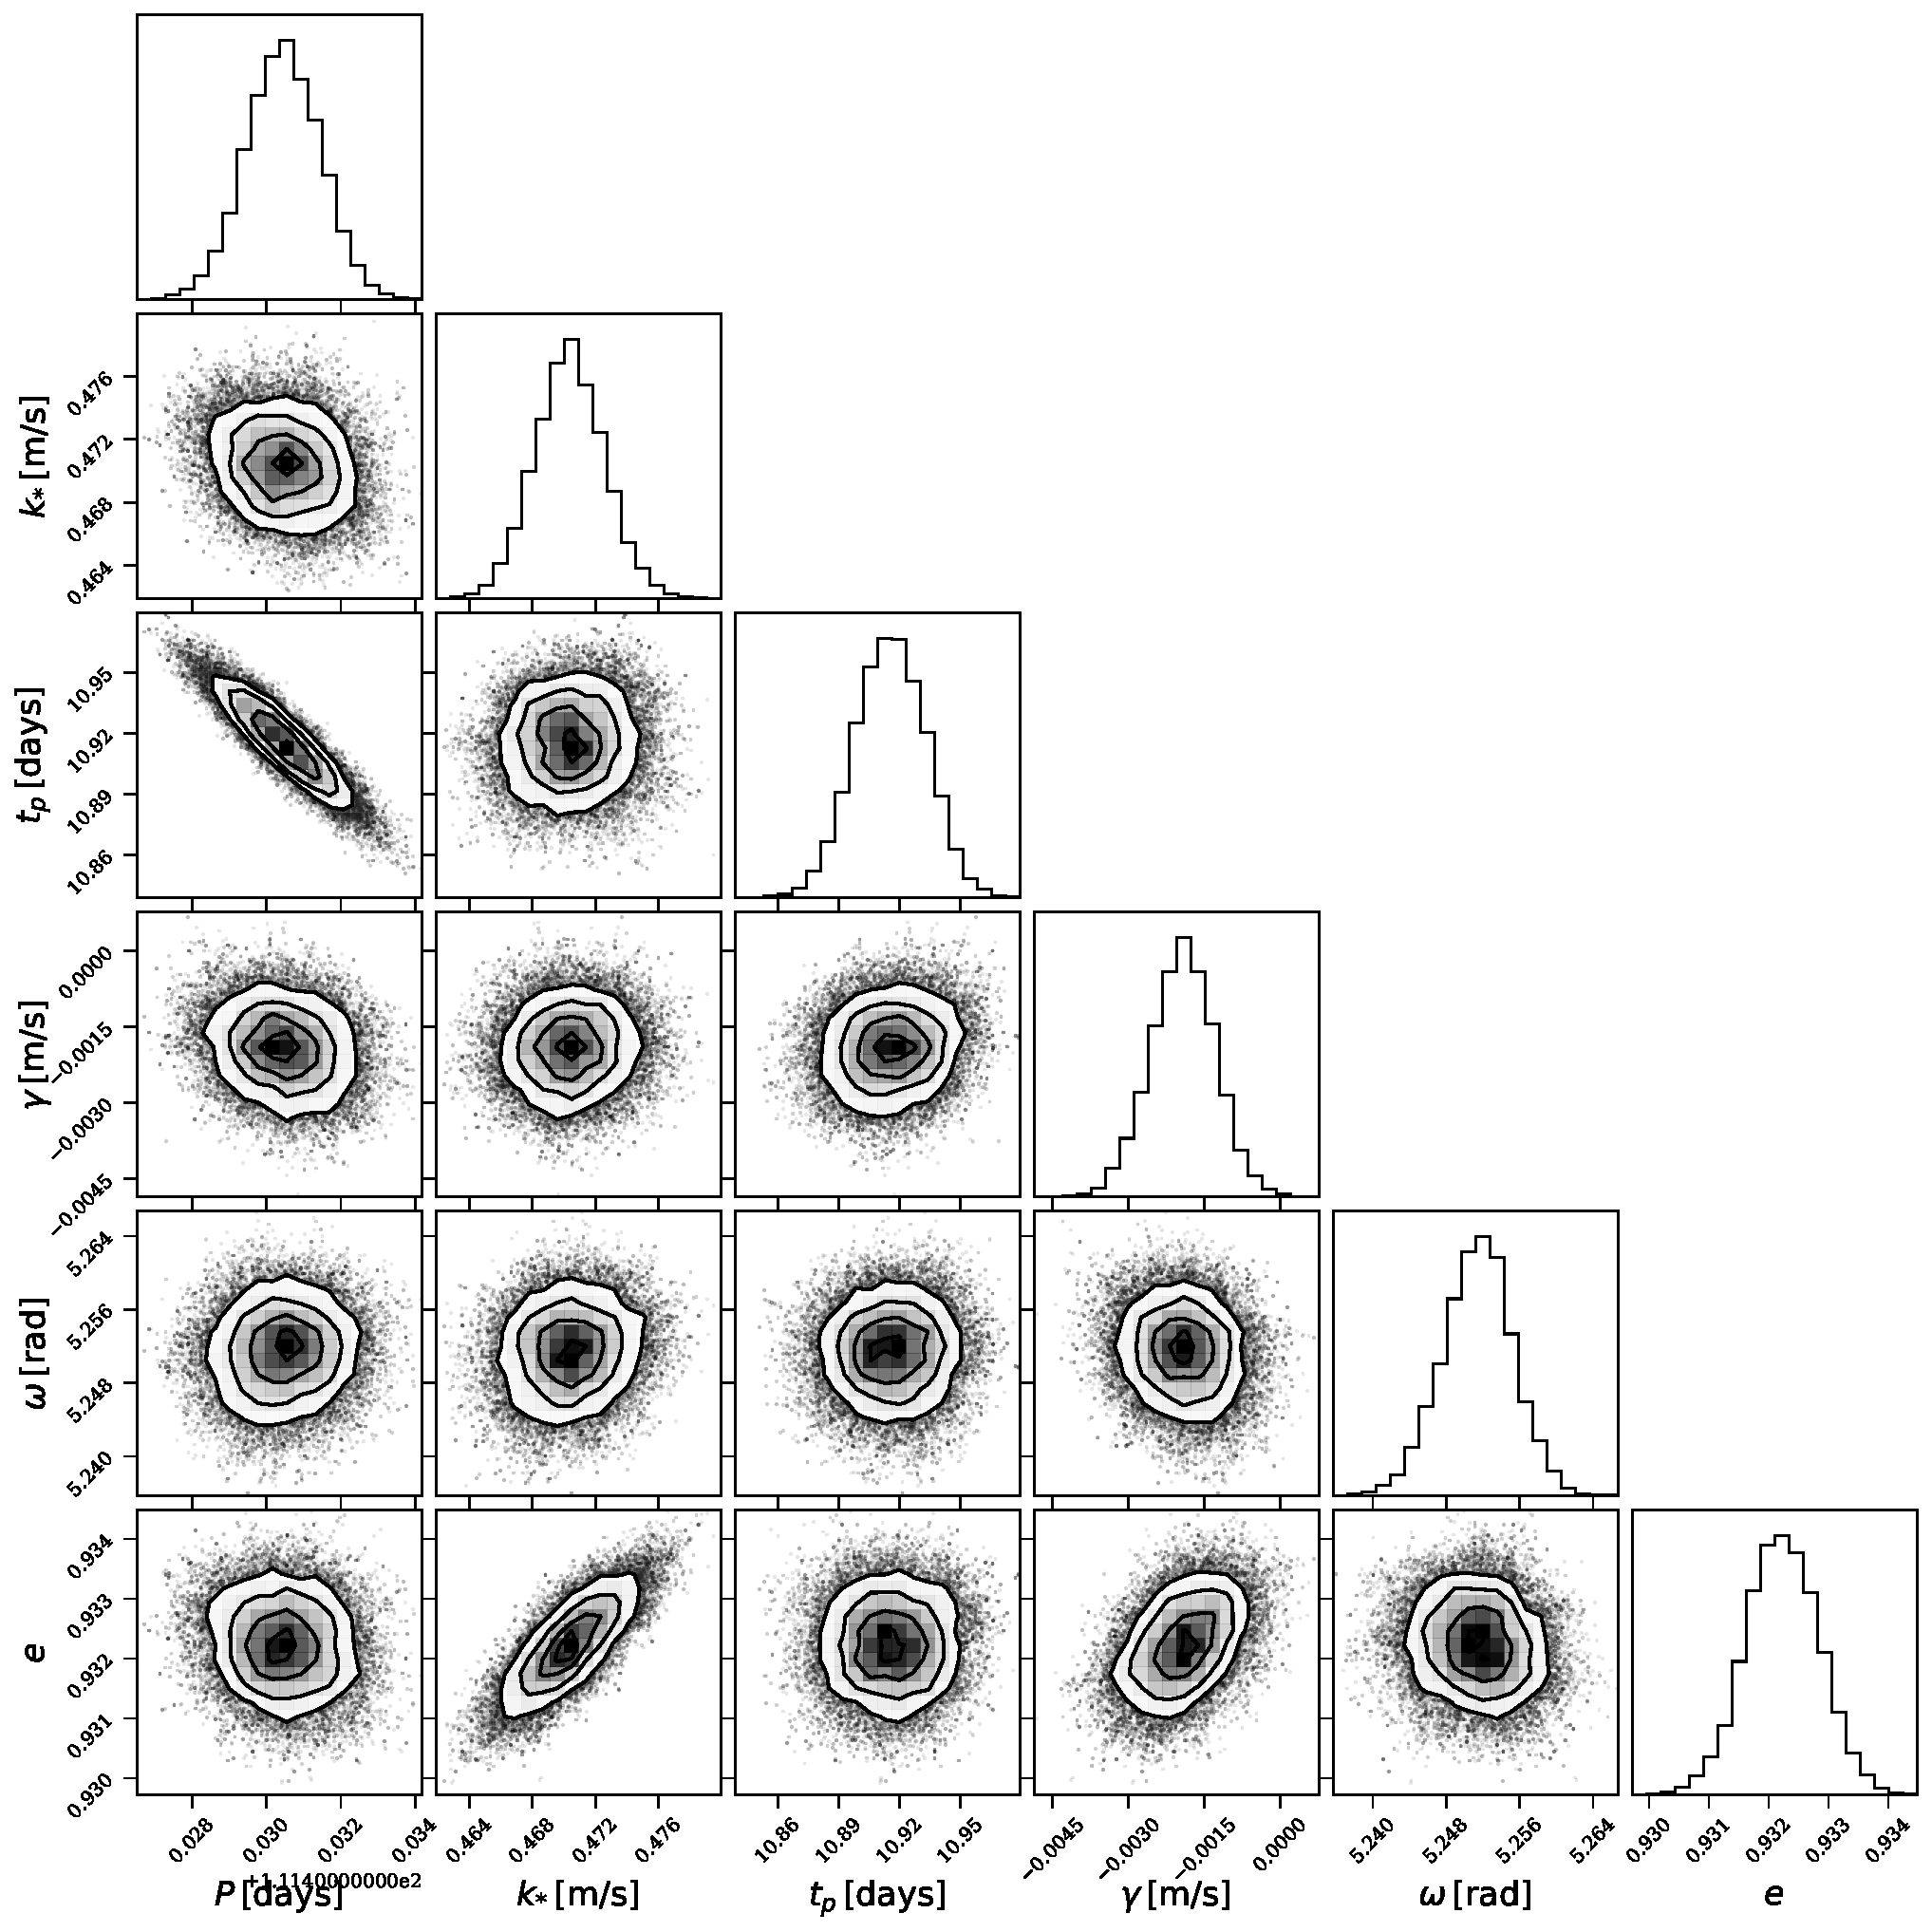
\includegraphics[width=\textwidth]{figures/mcmc_corner.pdf}
        \caption{Corner plot of the various planet parameters that I fit using \texttt{emcee}}
    \end{figure}

    \begin{figure}
        \centering
        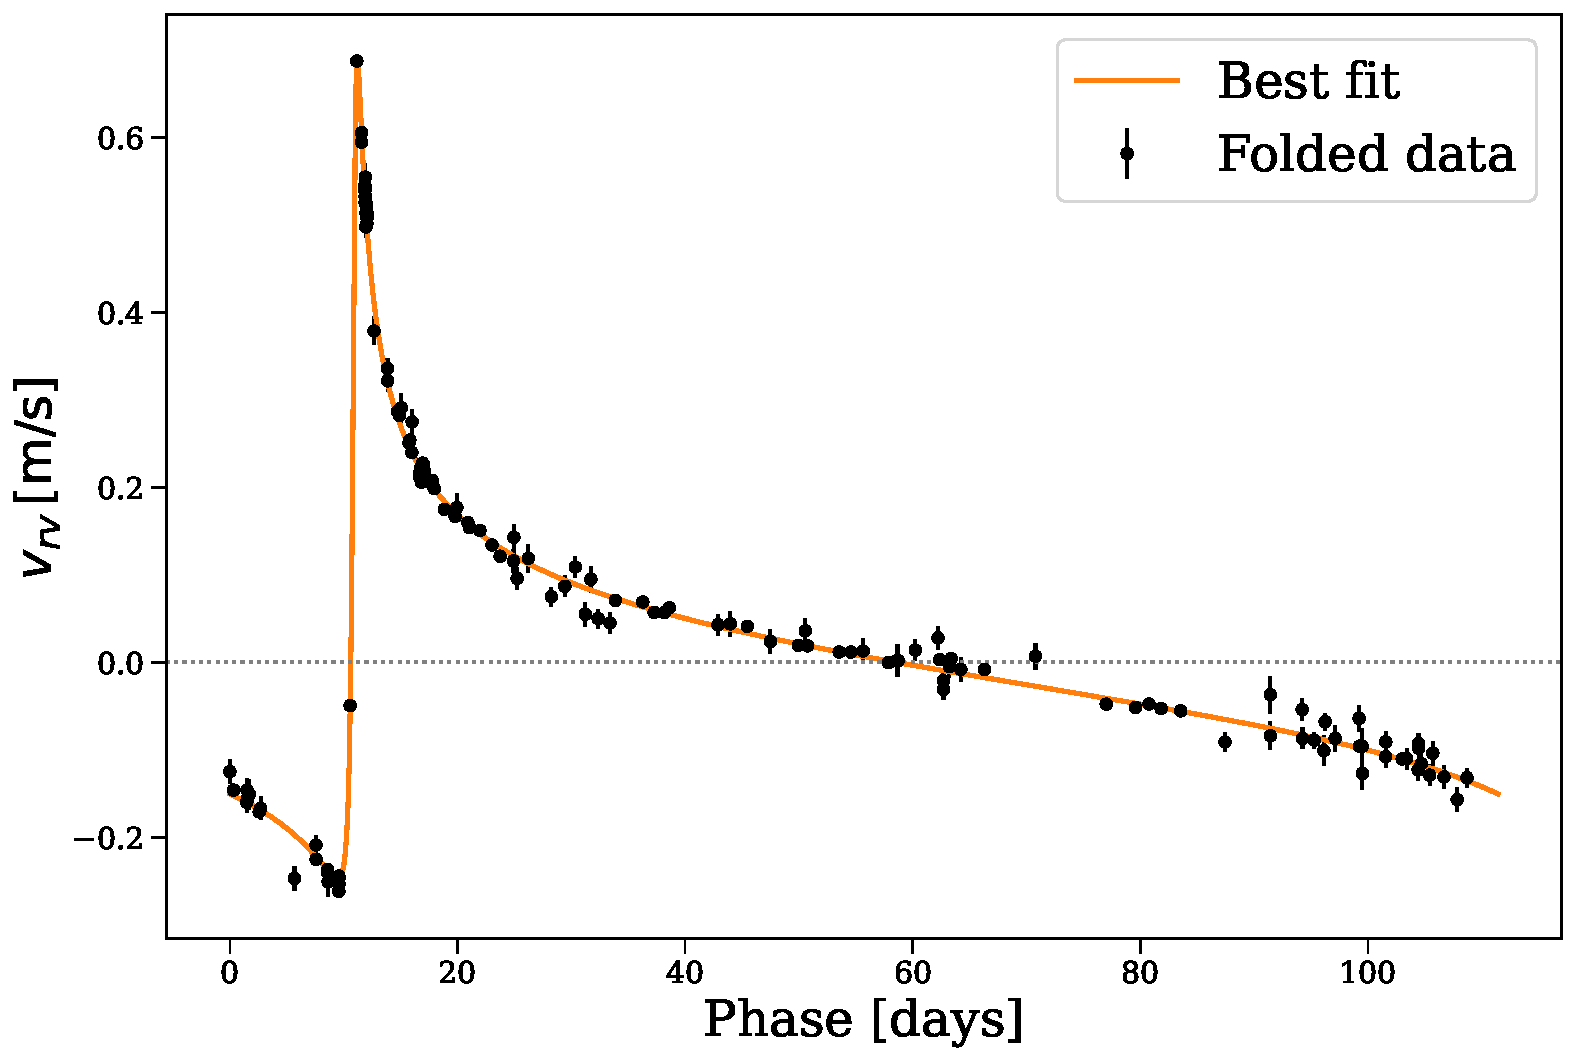
\includegraphics[width=0.7\textwidth]{figures/best_fit.pdf}
        \caption{Best fit to the data overlaid on top of the data folded using the best fitted period.}
    \end{figure}

    \begin{figure}
        \centering
        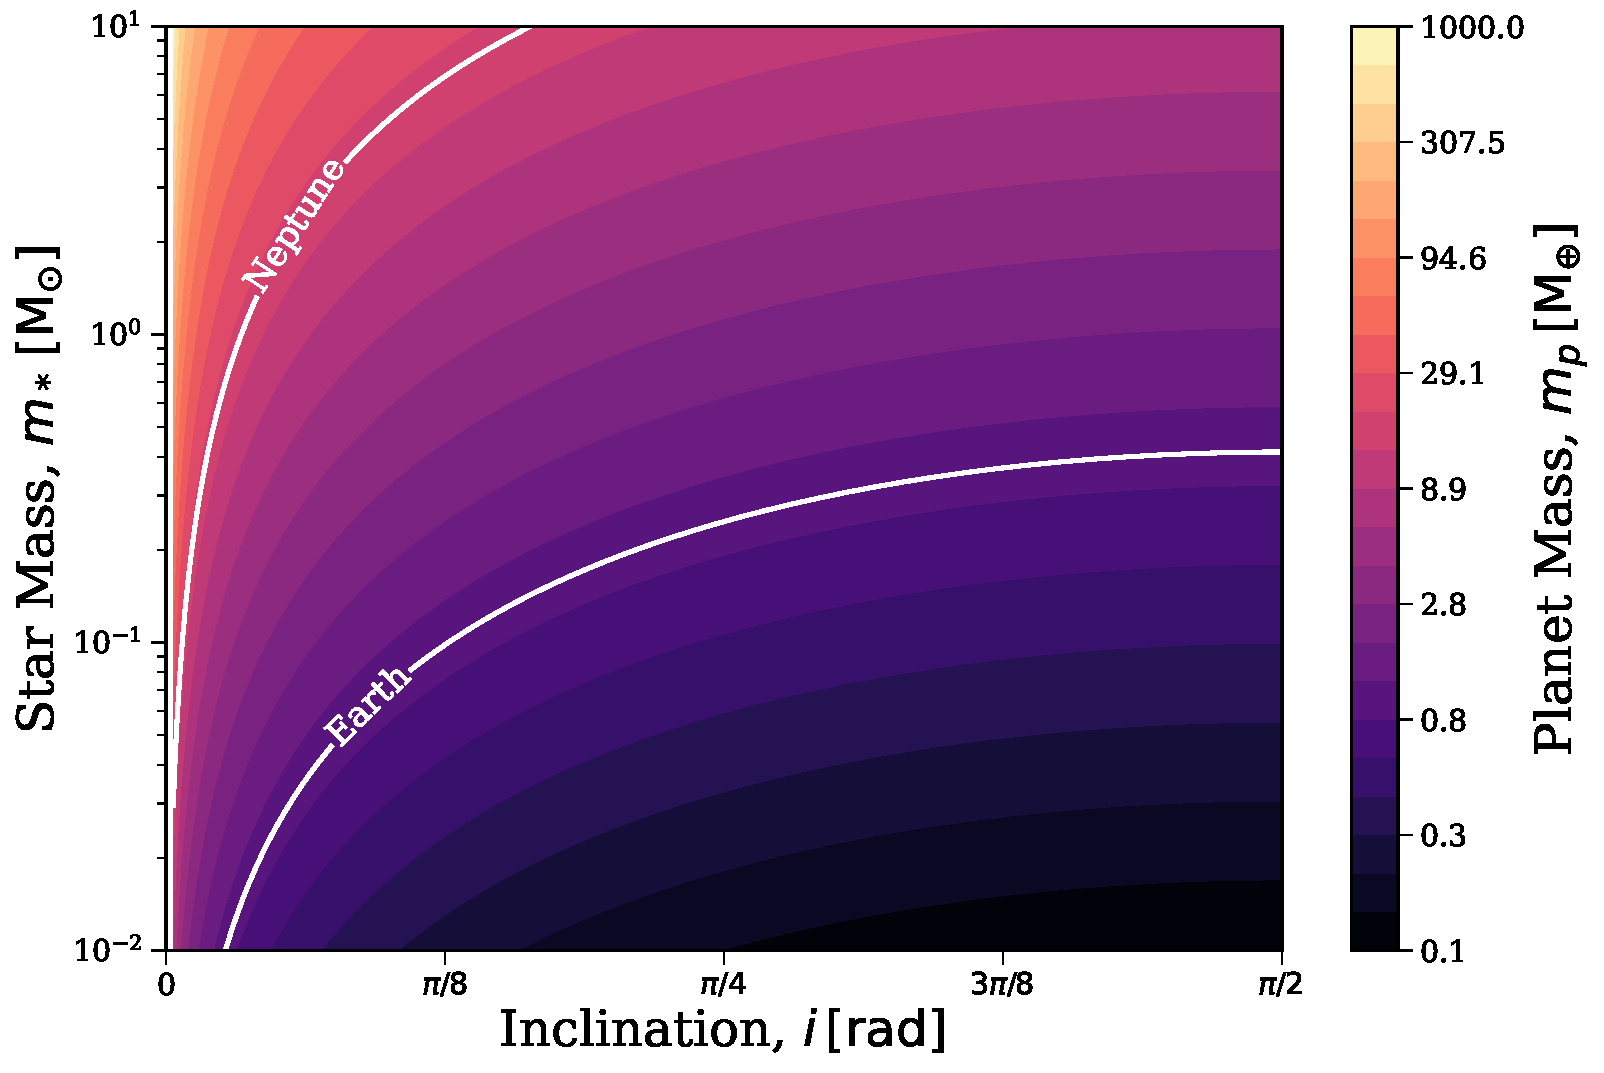
\includegraphics[width=0.7\textwidth]{figures/planet_mass.pdf}
        \caption{Contour plot of possible planet masses given the best fit parameters. Contours of shown for masses of Earth and Neptune.}
    \end{figure}
}


\end{document}

 